The Littlewood-Paley projections separate in a quantitative manner the different frequencies of a function or tempered distribution. We can describe this separation qualitatively by the following heuristics:
\begin{itemize}
	\item \textit{Low frequencies} $P_{\leq N} f$ are smooth/slowly varying/high regularity.
	
	\item \textit{High frequencies} $P_{\geq N} f$ are rough/quickly oscillating/low regularity.
	
	\item \textit{Medium frequencies} $P_N f$ share the properties of both high and low frequencies. 
\end{itemize}

\subsection{Uncertainty principle}

The \textit{uncertainty principle} states that one cannot simultaneously localise in one of physical or frequency space without uncertainty in the other. Formally, 
	\[ |\triangle x \cdot \triangle \xi| \gtrsim 1.\]
This manifests in the Littlewood-Paley theory as follows:	
\begin{itemize}
	\item \textit{Low frequencies} $P_{\leq N} f$ 
are approximately constant on spatial balls of radius $\ll 1/N$. 
	
	\item \textit{High frequencies} $P_{\geq N} f$ have approximate mean zero on spatial balls of radius $\gg 1/N$. 
	
	\item \textit{Medium frequencies} $P_N f$ share the properties of both high and low frequencies. 
\end{itemize}


\begin{figure}[h]
	\begin{center}
		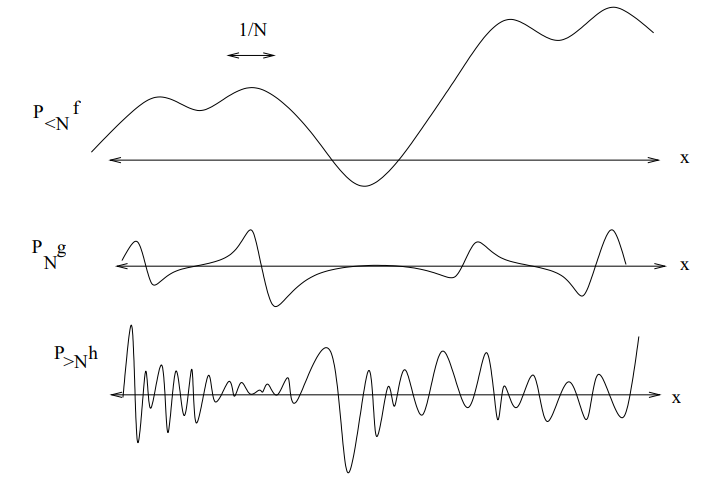
\includegraphics[scale =0.5]{uncertainty}
		\caption{Amplitudes of the projections to low, medium and high frequencies and their behavior at spatial scale $1/N$. This graphic is taken from \cite[Appendix A]{Tao2006}.}
	\end{center}
\end{figure}




\begin{proposition}[Local constancy for low frequencies]
	Let $k \in \N_0$, then 	
		\[ |\nabla^k f_{\leq N} (y)| \lesssim_{k, d} N^k \langle N(y - x) \rangle^d \cM f (x) \]
	uniformly for $f \in L^1_{\loc} (\R^d)$ and $N \in 2^\Z$. The analogous inequality holds replacing $f_N$ with $f_{\leq N}$. 
\end{proposition}

\begin{proof}
	By translation and scaling, we can assume without loss of generality that $x = 0$ and $N = 1$. The Littlewood-Paley projection can be written as a convolution with the kernel $\widecheck \phi \in \cS (\R^d)$. As the kernel and its derivatives are Schwartz, they can be bounded pointwise by $|\nabla^k \widecheck \phi (x)| \lesssim \langle x \rangle^{-100d}$. Thus
		\begin{align*}
			 |\nabla^k P_{\leq 1} f (y)|
			 	&\lesssim \int_{\R^d} \frac{|f(z)|}{\langle  y - z \rangle^{100d}} \, dz.
		\end{align*}	
	We divide the integral up into two regions. In the region $|z| \lesssim \langle y\rangle$, we crudely estimate
		\begin{align*}
			\int_{|z| \lesssim |y|}  \frac{|f(z)|}{\langle  y - z \rangle^{100d}} \lesssim \int_{|z| \lesssim |y|} |f(z)| \, dz \lesssim \langle y \rangle^d \cM f(0).
		\end{align*}
	In the region $|z| \gg \langle y\rangle$, the denominator can be estimated as $\langle y - z \rangle^{-100d} \sim \langle z \rangle^{-100d}$, then we decompose the region into dyadic annuli of radii $R \in 2^\N$ to write	
		\begin{align*}
			\int_{|z| \gg |y|} \frac{|f(z)|}{\langle  y - z \rangle^{100d}} \, dz
						&\lesssim \sum_{\substack{R \in 2^\N}} \int_{R \leq |z| \leq 2R} \frac{|f(z)|}{\langle z \rangle^{100d}} \, dz \\
						&\sim \sum_{\substack{R \in 2^\N}} R^{-100d}\int_{|z| \leq 2R} |f(z)| \, dz\lesssim \sum_{\substack{R \in 2^\N}} \langle R \rangle^{-99d} \cM f(0) \lesssim \cM f(0).
				\end{align*}
	This proves the pointwise inequality. 
\end{proof}

The fact that high frequencies have approximate mean zero on large balls is less useful, so we only sketch how to formalise the principle. Choose $\phi_{\lesssim N} \in \cS (\R^d)$ with disjoint Fourier support from $P_{\geq N} f$, then 
	\[ \int_{\R^d} \widecheck{\phi_{\lesssim N}} f_{\geq N} \, dx = 0 \]
by Plancharel. The inverse Fourier transform $\widecheck{\phi_{\lesssim N}} \in \cS (\R^d)$ is a Schwartz function adapted to the ball $B_{1/N} (0)$; modulating in frequency space allows us to adapt it to any ball $B_{1/N} (x_0)$. The mass outside of this ball, modulo scaling the radius by a constant, is negligible, hence
	\[ \int_{B_{C/N} (x_0)} f_{\geq N} \, dx \approx 0. \]

\subsection{Bernstein's inequalities}

There are two obstructions to moving between $L^p$-spaces: growth of singularities and decay at infinity. At one end, $L^\infty$-functions have no singularities and no decay at infinity, and at the other end, $L^1$-functions can have large singularities and a lot of decay at infinity. Projecting to low frequencies ``smooths'' the singularities, so we can ``pay'' some of this smoothing to control a higher $L^q$-space by a lower $L^p$-space. 

\begin{proposition}[Bernstein's inequalities]\label{prop:bernstein}
	For $1 \leq p \leq q \leq \infty$ and $f \in L^p (\R^d)$, then 
	\begin{align*}
					||f_N||_{L^q} 
						&\lesssim_{p, q} N^{\frac{d}{p} - \frac{d}{q}} ||f_N||_{L^p}, \\
					||f_{\leq N}||_{L^q} 
						&\lesssim_{p, q} N^{\frac{d}{p} - \frac{d}{q}} ||f_{\leq N}||_{L^p}. 
				\end{align*}
\end{proposition}

\begin{proof}
	Let $1 \leq r \leq \infty$ satisfy $\tfrac1p + \tfrac1r = \tfrac1q + 1$, then by Young's convolution inequality and a change of variables $Nx = y$, we have the inequality
	\begin{align*}
		|| P_N f ||_{L^q} = || f * \widecheck{\psi_N} ||_{L^p} \leq ||f||_{L^p} ||N^d \widecheck \psi(Nx)||_{L^r_x} = N^{d - \frac{d}{r}} ||f||_{L^p} ||\widecheck \psi ||_{L^r_y} \sim N^{\frac{d}{p} - \frac{d}{q}} ||f||_{L^p}.
	\end{align*}
	To obtain $f_N$ instead of $f$ on the right, observe that the same proof holds replacing $P_N$ with the fattened projection $\widetilde{P_N}$. Since $\widetilde{P_N} P_N = P_N$, replacing $f$ with $P_N f$ completes the proof. Arguing similarly furnishes the inequality replacing $f_N$ with $f_{\leq N}$. 
\end{proof}

\begin{remark}
	Compare with the dual phenomenon of localising in physical space, where if $1 \leq p \leq q \leq \infty$, applying Holder's inequality gives
		\[ ||\phi_{\leq N} f||_{L^p} \lesssim N^{\frac{d}{p} - \frac{d}{q}} ||\phi_{\leq N} f||_{L^q}. \]
	Applying a cut-off gives decay at infinity, which allows us to ``pay'' this decay to control a lower $L^p$-space by a higher $L^q$-space. 	
\end{remark}

\begin{remark}
	It is instructive to use the uncertainty principle to justify Bernstein's inequality. Suppose most of the $L^p$ and $L^q$-mass is located in a ball of radius $O(1)$, and recall low frequencies are locally constant at scales $\ll 1/N$. Hence we can approximate $f_{\leq N}$ by a function on the discrete space $N^d$, where we have the following discrete analogue of Bernstein's inequality,
		\[ ||f||_{\ell^q (N^d)} \lesssim N^{\frac{d}{p} - \frac{d}{q}} ||f||_{\ell^p (N^d)}. \]
\end{remark}


\subsection{Sobolev-Bernstein inequalities}

When applying for example the solid gradient $|\nabla|^s$ to a Littlewood-Paley projection and examining the symbol in frequency space, we can formally justify the following heuristics:
\begin{itemize}
	\item \textit{Low frequencies} are diminished by positive order differential operators and accentuated by negative orders, 
		\[ |\nabla|^s P_{\leq N} f \lesssim N^s P_{\leq N } f \qquad \text{for $s \geq 0$}.\] 
	
	\item \textit{High frequencies} are accentuated by positive order differential operators and diminished by negative orders,
		\[ |\nabla|^{s} P_{\geq N} f \lesssim N^{s}P_{\geq N} f \qquad \text{for $s \leq 0$}.\] 
	
	\item \textit{Medium frequencies} share the properties of both high and low frequencies,  	
		\[ |\nabla|^s P_{\leq N} f \sim N^s P_N f \qquad \text{for $s \in \R$}.\] 
\end{itemize}
These heuristics can be made rigorous to prove the \textit{Sobolev embedding inequalities}. Morally, if one can prove Sobolev embedding for a Littlewood-Paley piece, one can prove it for a generic function via summing. As such, we introduce


\begin{lemma}[Sobolev-Bernstein inequalities] For $f \in L^p (\R^d)$, 
				\begin{alignat*}{2}
					|| |\nabla|^s f_{\leq N}||_{L^p} 
						&\lesssim N^s ||f_{\leq N}||_{L^p}, &&\qquad\text{if }s > 0 \text{ and } 1 \leq p < \infty, \\
					|| |\nabla|^s f_{\geq N}||_{L^p} 
						&\lesssim N^s ||f_{\geq N}||_{L^p}, &&\qquad\text{if }s < 0 \text{ and } 1 \leq p < \infty \\
					|| |\nabla|^s f_N||_{L^p} 
						&\sim N^s ||f_N||_{L^p}, &&\qquad \text{if }s \in \R \text{ and } 1 \leq p \leq \infty
				\end{alignat*}			
		The endpoint cases $p = \infty$ for the first two inequalities hold for $f \in C_0 (\R^d)$. 
\end{lemma}

\begin{proof}
	Let 
		\[ \chi (\xi) := |\xi|^s \psi (\xi), \qquad \chi_N (\xi) := \chi (\xi/N). \]
	Observe that $\chi \in \cS (\R^n)$ since $\psi$ vanishes in a neighborhood of the origin. Then by Young's convolution inequality and the change of variables $Nx = y$, we have
		\[ || |\nabla|^s f_N||_{L^p} = || ({|\xi|^s \psi (\xi/N)})^{\vee} * f ||_{L^p} = N^s ||\widecheck{\chi_N} * f||_{L^p} \leq N^s ||f||_{L^p} ||N^d \widecheck{\chi} (N x)||_{L^1_x} = N^s ||f||_{L^p} ||\widecheck \chi(y)||_{L^1_y}. \]	
	The inequality continues to hold using instead the fattened Littlewood-Paley projections, so arguing as we did in Bernstein's inequality, we can replace $f$ with $f_N$ on the right-hand side. To obtain the reverse inequality, note the previous argument holds for the fattened projections. Hence, since Fourier multipliers commute and $\widetilde{P_N} P_N = P_N$,
		\[ ||f_N||_{L^p} = || |\nabla|^{-s} \widetilde{P_N} |\nabla|^s f_N||_{L^p} \lesssim N^{-s} || |\nabla|^s f_N||_{L^p}.  \]
	Rearranging furnishes the result. 	

	To prove the inequalities, we remark that the representation formulas $\sum_{K \leq N} f_K = f_{\leq N}$ and $\sum_{K \geq N} f_K = f_{\geq N}$ hold in $L^p (\R^d)$ for $1 < p < \infty$ and in the case $p = 1$ when $f$ has zero mean, see the following section for proofs. It follows from the triangle inequality that
		\[	|| |\nabla|^s f_{\leq N} ||_{L^p} \leq \sum_{K \leq N} || | \nabla|^s f_K||_{L^p} \sim \sum_{K \leq N} K^s ||f_K||_{L^p} \lesssim N^s ||f_{\leq N} ||_{L^p}\]
	for $s > 0$ and $1 \leq p < \infty$ and
		\[	|| |\nabla|^s f_{\geq N} ||_{L^p} \leq \sum_{K \geq N} || | \nabla|^s f_K||_{L^p} \sim \sum_{K \geq N} K^s ||f_K||_{L^p} \lesssim N^s ||f_{\geq N} ||_{L^p}\]
	for $s < 0$ and $1 \leq p < \infty$. 
\end{proof}


\subsection{Localised estimates}

When studying partial differential equations, we often times only want to look at a solution locally.  The standard way of doing this is to multiply by a cut-off function $\chi \in C^\infty_c (\R^d)$ adapted to a spatial ball of radius $R$. By the uncertainty principle, its Fourier transform should be adapted to a frequency ball of radius $R^{-1}$, thus multiplication by $\chi$ ``almost'' commutes with $P_N$ for $RN \gg 1$. Formally, 
	\[ [P_N, \chi] \approx O (N^{-1} \nabla \chi \widetilde{P_{\leq N}}).  \]

\begin{proposition}[Commutator estimate]
	Let $1 \leq p \leq \infty$ and $\chi \in C^\infty_c (\R^d)$ is a smooth cut-off. For $R > 0$, set $\chi_R (x) := \chi (x/R)$, then for any $k \geq 1$ we have 
		\[ || [P_N, \chi_R] f||_{L^p} \lesssim (RN)^{-1} ||\nabla \chi||_{L^\infty} || {P_{\leq 2N}} f||_{L^p} +  (RN)^{-k} || |\nabla|^k \chi||_{L^\infty}||f||_{L^p} .\]
\end{proposition}

\begin{proof}
	By scaling, assume without loss of generality $R  = 1$. We perform a paraproduct decomposition, inserting the expansions $\chi = \sum_A \chi_A$ and $f = \sum_B f_B$ and separating between high-low, high-high, and low-high interactions,
		\begin{align*}
			[P_N, \chi] f 
				&= P_N (\chi f) - \chi P_N f\\
				&= \left(\sum_{\substack{B \geq 4N \\ A \leq B/4}} + \sum_{\substack{B \geq 4N \\ A \geq B/2}} + \sum_{\substack{B \leq 2N \\ A \in 2^\Z}} \right) P_N (P_A \chi P_B f) - P_A \chi P_N P_B f.
		\end{align*}	
	Notice that the high-low summands vanish, since in this frequency regime $P_A \chi P_B f$ and $P_B f$ have Fourier supports at high frequencies $|\xi| \geq 2N$ and thus vanish when applying the projection $P_N$. For the high-high summand, again $P_N P_B f = 0$, while the term $P_A \chi P_B f$ can be dealt with by using smoothness of the cut-off to gain decay via Sobolev-Bernstein, 
		\begin{align*}
			 \sum_{\substack{B \geq 4N \\ A \geq B/2}} || P_N  (P_A \chi P_B f) ||_{L^p}
			 	&\lesssim \sum_{\substack{B \geq 4N \\ A \geq B/2}}  || | P_A \chi||_{L^\infty} || P_B f ||_{L^p} \\
			 	&\lesssim \sum_{\substack{B \geq 4N }} \sum_{A \geq B/2} A^{-k} || |\nabla|^k \chi||_{L^\infty} ||f||_{L^p}  \lesssim N^{-k} || |\nabla|^k \chi||_{L^\infty} ||f||_{L^p} . 
		\end{align*}	 
	It remains to estimate the low-high sum. Changing variables, we can write pointwise	
		\begin{align*}
			P_N (\chi P_{\leq 2N} f) (x) 
				&= \int_{\R^d} \widecheck \phi (y) \chi (x - y/N) P_{\leq 2N} f(x - y/N) \, dy,\\
			\chi P_N P_{\leq 2N} f (x)
				&= \int_{\R^d} \widecheck \phi (y) \chi (x) P_{\leq 2N} f (x - y/N) \, dy.
		\end{align*}
	By the fundamental theorem of calculus, we can estimate the difference $|\chi(x) - \chi(x - y/N)| \lesssim |y| N^{-1} ||\nabla \chi||_{L^\infty}$. It follows then from Minkowski's integral inequality and integrability of $y \widecheck \phi \in \cS (\R^d)$ that 
		\begin{align*}
			||P_N (\chi P_{\leq 2N} f) - \chi P_N P_{\leq 2N} f||_{L^p}
				&\leq N^{-1} ||\nabla \chi||_{L^\infty} ||P_{\leq 2N} f||_{L^p}.
		\end{align*}	
	This completes the proof. 
\end{proof}	

\begin{remark}
	The estimate can be further refined so that the $L^p$-norms on the right are localised by writing $\chi = \widetilde \chi \chi$, where $\widetilde \chi \equiv 1$ on the support of $\chi$. 
\end{remark}

In a similar spirit, we have a spatially localised version of Bernstein's inequality, see for example \cite{Tao2020} and \cite{Palasek2022} for applications to the Navier-Stokes equations: 

\begin{proposition}[Localised Bernstein's inequality]
	Let $\Omega \subseteq \R^d$ be a domain and $N \in 2^\Z$. For any $R \geq 1$ and $k \gg 1$, 
		\[ || P_N f ||_{L^{q_1} (\Omega)} \lesssim_{p_1, p_2, q_1, q_2, k} N^{\frac{d}{p_1} - \frac{d}{q_1}} ||f||_{L^{p_1} (B_R (\Omega))} + (RN)^{-k} |\Omega|^{\frac{1}{q_1} - \frac{1}{q_2}} N^{\frac{d}{p_2} - \frac{d}{q_2}} ||f||_{L^{p_2} (\R^d)}  \]
	whenever $1 \leq p_1 \leq q_1 \leq \infty$ and $1 \leq p_2 \leq q_2 \leq \infty$ such that $q_1 \leq q_2$. 
\end{proposition}

\begin{proof}
	We decompose $f = f \mathbb 1_{B_R (\Omega)} + f \mathbb 1_{\R^d \setminus B_R (\Omega)}$. The component supported on $B_R (\Omega)$ can be estimated by the first term on the right via Bernstein's inequality, it remains to show that $f =  f \mathbb 1_{\R^d \setminus B_R (\Omega)}$ supported on the complement $\R^d \setminus B_R (\Omega)$ is controlled by the second term on the right. By Holder's inequality, 
		\begin{align*}
			|| P_N f ||_{L^{q_1} (\Omega)} \leq |\Omega|^{\frac{1}{q_1} - \frac{1}{q_2}} || P_N f||_{L^{q_2} (\Omega)}. 
		\end{align*}
	For $x \in \Omega$, we can replace the kernel to its restriction to $|y| \geq R$, writing $P_N f(x) = (f * \mathbb 1_{|y| \geq R}\widecheck \psi_N) (x)$. Following the proof of Bernstein's inequality, we apply Young's convolution inequality and estimate $\widecheck \psi \in \cS (\R^d)$ by $|\widecheck \psi (y)| \lesssim_k \langle y \rangle^{-k}$, furnishing
		\[ ||P_N f||_{L^{q_2} (\Omega)} \leq  ||\widecheck \psi_N||_{L^r (|y| \geq R)} ||f||_{L^{p_2} (\R^d)} \lesssim_k (RN)^{-k} N^{\frac{d}{p_2} - \frac{d}{q_2}} ||f||_{L^{p_2} (\R^d)}.  \]
	This completes the proof. 
\end{proof}

